%
% budgets.tex
%
% Copyright (C) 2021 by SpaceLab.
%
% GOLDS-UFSC Documentation
%
% This work is licensed under the Creative Commons Attribution-ShareAlike 4.0
% International License. To view a copy of this license,
% visit http://creativecommons.org/licenses/by-sa/4.0/.
%

%
% \brief Budgets and mission analysis chapter.
%
% \author Gabriel Mariano Marcelino <gabriel.mm8@gmail.com>
%
% \institution Universidade Federal de Santa Catarina (UFSC)
%
% \version 0.2.0
%
% \date 2020/06/11
%

\chapter{Technical Budgets and Mission Analysis} \label{ch:budgets}

This chapter presents a general analysis of the mission, such as a preliminary analysis of the satellite's estimated orbit, estimated lifetime, and the amount of data exchanged along its operation.

Another type of analysis presented is the satellite budgets, such as the power and link budgets.

\section{Requirements}

The mission requirements are listed next:

\begin{enumerate}
    \item The power system must be able to harvest solar energy.
    \item The power system must be able to store energy for use when GOLDS-UFSC is eclipsed.
    \item The power system must supply energy to all other modules.
    \item The data handling system must communicate with the other modules and store their data.
    \item The communications system must send a beacon signal periodically using VHF radio.
    \item The communications system must send the CubeSat telemetry using UHF radio.
    \item The communications system must be able to receive telecommands and respond to them accordingly.
    \item The attitude system must be able to perform a 1-axis stabilization of the CubeSat.
    \item GOLDS-UFSC must be able to receive and execute a shutdown telecommand, therefore ceasing all transmissions.
    \item The downlink transmissions must be done once at a time, either telemetry or beacon.
    \item The ground station must operate under the proper radio frequency communication licenses.
    \item GOLDS-UFSC must comply with international and Brazilian radio license agreements and restrictions.
    \item The team must build and operate a ground station for full communication with GOLDS-UFSC.
    \item GOLDS-UFSC must be capable of sustaining the primary payload (EDC) operation.
    \item The service module and payload must employ materials and components that do not compromise or damage LIT/INPE test facilities.
    \item The satellite must reenter the Earth's atmosphere within 25 years.
    \item It is recommended that the satellite be placed in an orbit up to 500 km.
\end{enumerate}


\section{Orbit Parameters and Analysis}

% To define the orbit parameters and 
To simulate the behavior of the satellite during its operation, the software SimCube developed at the SpaceLab was used. It is important to emphasize that the results presented in this chapter are preliminary, since the actual orbit parameters are yet to be defined and are subject to market availability.

%the GMAT\nomenclature{\textbf{GMAT}}{\textit{General Mission Analysis Tool.}} software was used \cite{gmat}.
The orbit parameters were based on the FloripaSat-1 TLE\nomenclature{\textbf{TLE}}{\textit{Two-Line Element.}}, but with a lower altitude. These parameters can be seen in \autoref{tab:orbit-parameters}.

\begin{table}[!h]
    \centering
    \begin{tabular}{lcc}
        \toprule[1.5pt]
        \textbf{Parameters} & \textbf{Value} & \textbf{Unit} \\
        \midrule
        Apogee                & 550           & km \\
        Eccentricity            & 0.0015051     & - \\
        Inclination             & 97.9750       & $^{\circ}$ \\
        RAAN                    & 85.5100       & $^{\circ}$ \\
        Arg. of Perigee         & 194.87        & $^{\circ}$ \\
%        True                      & 99,8877       & $^{\circ}$ \\ %Essa linha não precisa
        \bottomrule[1.5pt]
    \end{tabular}
    \caption{Initial orbit parameters (adapted from FloripaSat-1).}
    \label{tab:orbit-parameters}
\end{table}

The parameters of the simulation were based on \cite{en13246691} and can be seen below:

\begin{itemize}
    \item Force model for gravitational field: ``\textit{Earth Gravitational Model 1996 (EGM96)}''
%    \item Propagator: ``\textit{PrinceDorman78}''
    \item Drag coefficient: 2.2
    \item Drag atmosphere model: ``\textit{NRLMSISE-00}''
    \item Epoch: 01 Jan 2022 11:59:28.000
\end{itemize}

The \autoref{fig:fsat2-gmat} shows the 3D representation of the GOLDS-UFSC orbit simulation, while \autoref{fig:fsat2-gmat-groundtrack} shows the ground track of a regular orbit obtained with the GMAT\nomenclature{\textbf{GMAT}}{\textit{General Mission Analysis Tool.}} software \cite{gmat}.

\begin{figure}[!ht]
    \begin{center}
        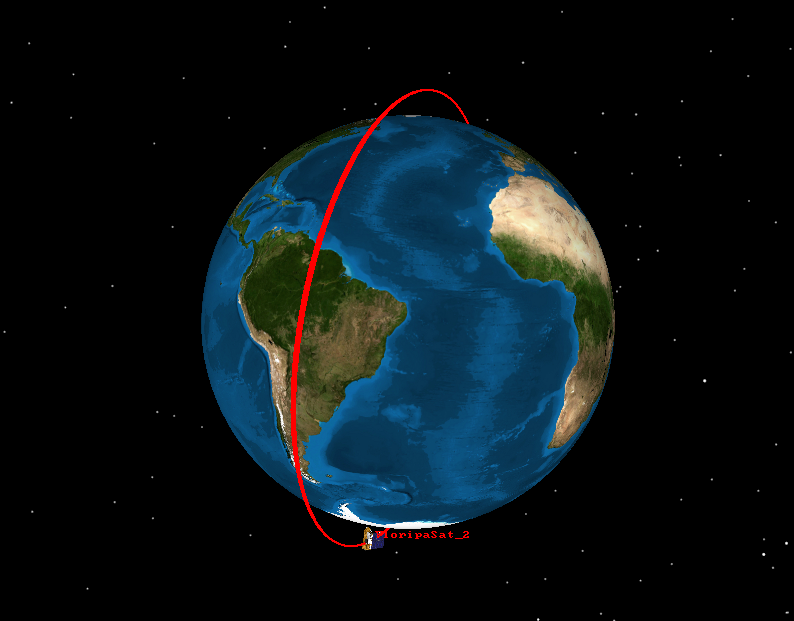
\includegraphics[width=0.6\textwidth]{figures/fsat2-gmat.png}
        \caption{GOLDS-UFSC orbit simulation on GMAT.}
        \label{fig:fsat2-gmat}
    \end{center}
\end{figure}

\begin{figure}[!ht]
    \begin{center}
        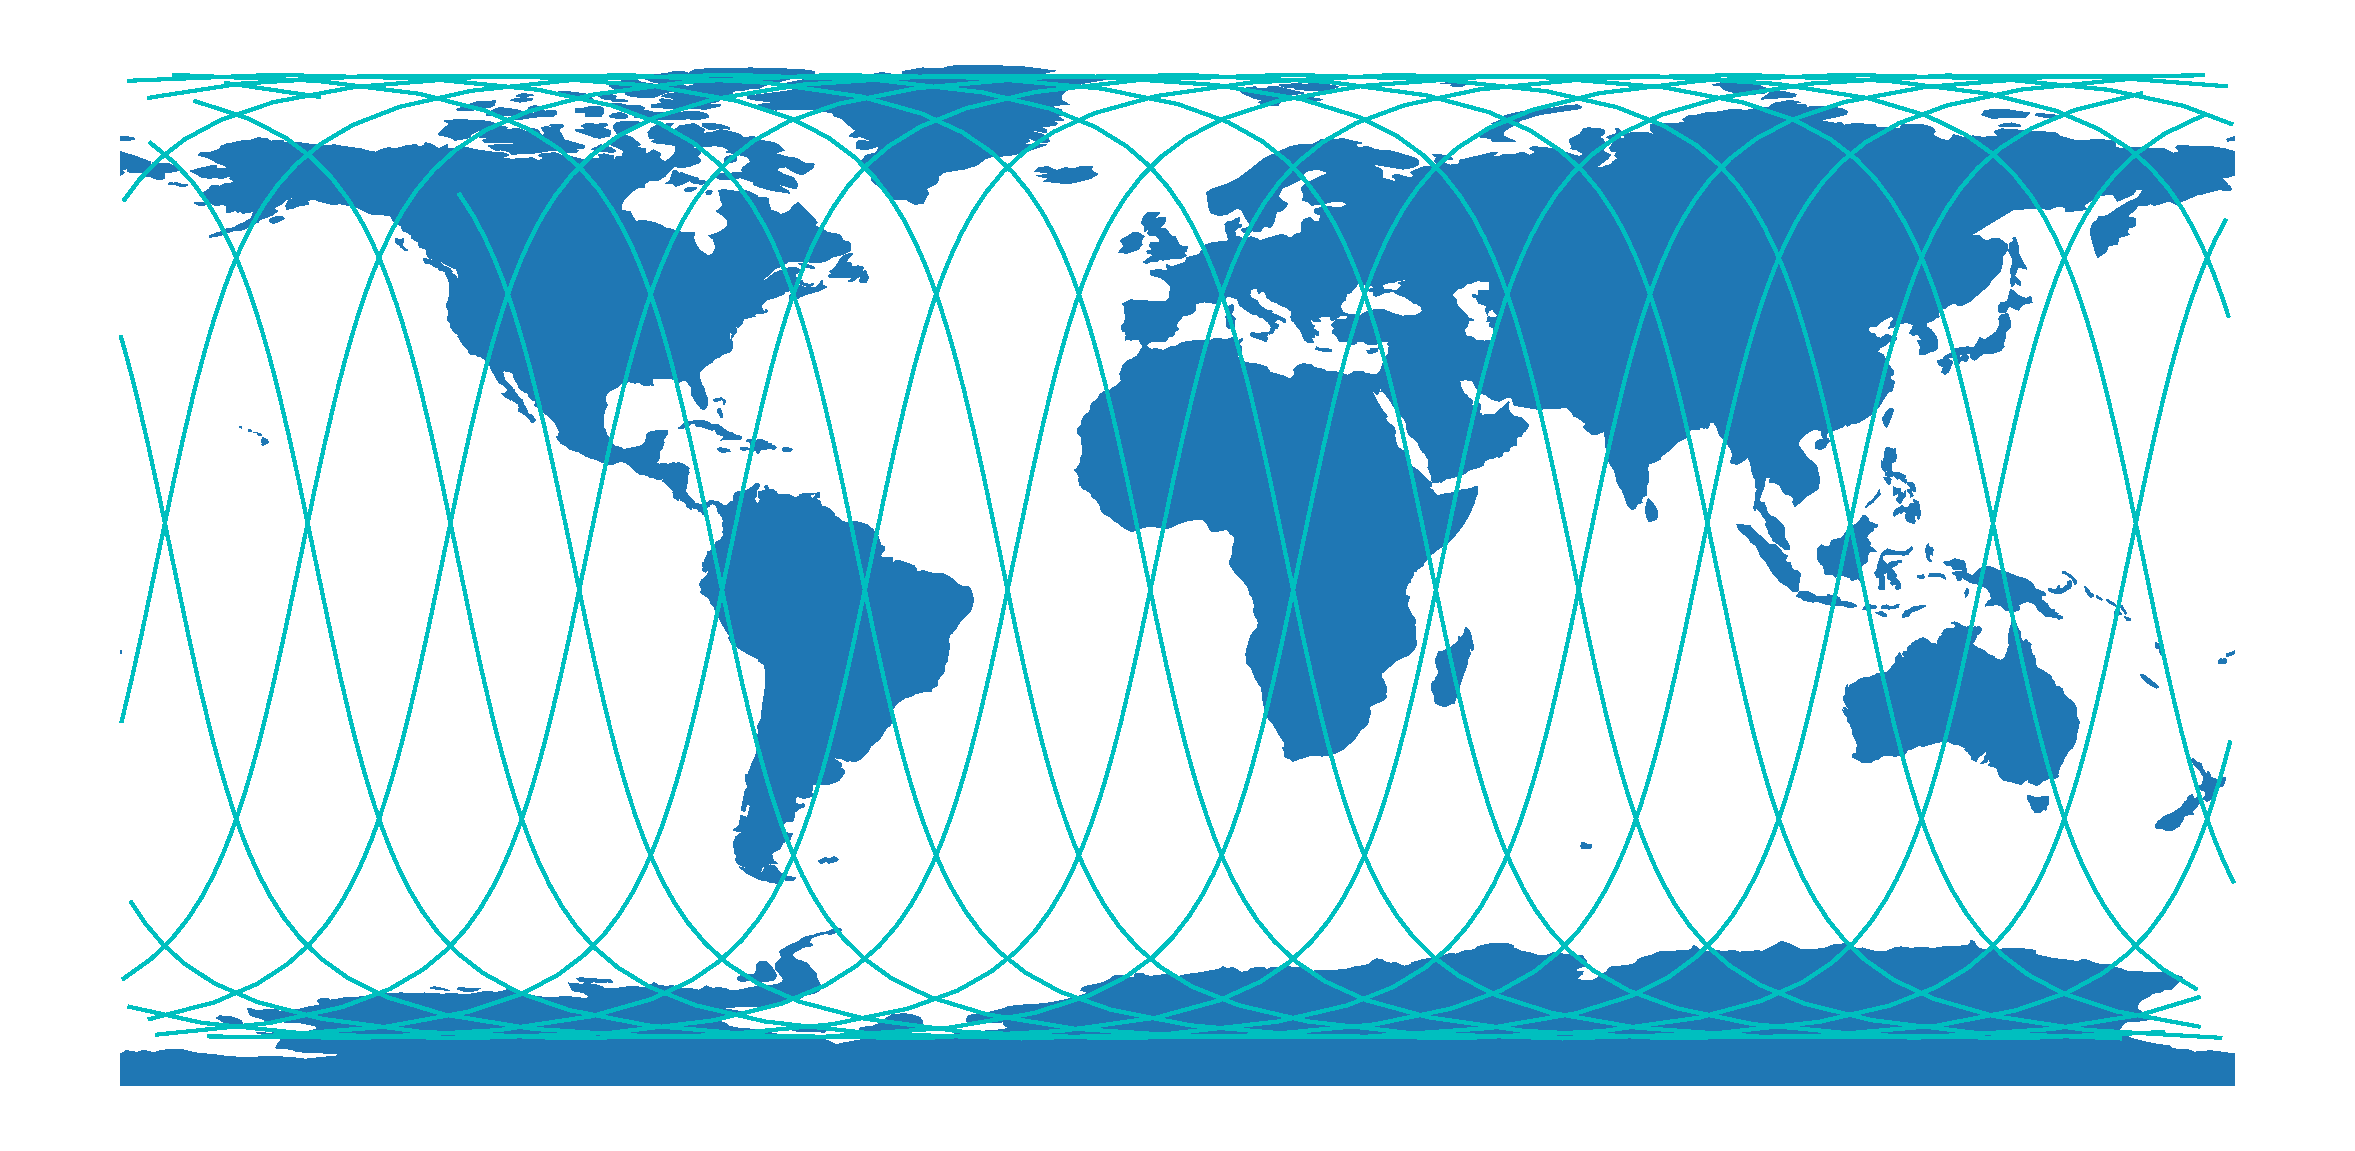
\includegraphics[width=\textwidth]{figures/fsat2-gmat-groundtrack.pdf}
        \caption{GOLDS-UFSC simulated groundtrack.}
        \label{fig:fsat2-gmat-groundtrack}
    \end{center}
\end{figure}

The next sections present some analysis based on the results obtained from the simulations performed with SimCube.% executed on GMAT.

%The source files of the GMAT simulation are available in \cite{fsat2-mechanical}.

\subsection{Lifetime Analysis}

Considering the same parameters of FloripaSat-1, but with an initial altitude of 550 km, the simulations on SimCube showed that the satellite decays approximately in 2183 days ($\cong$ 6 years), as can be seen in \autoref{fig:lifetime-analysis}.

\begin{figure}[!ht]
    \begin{center}
        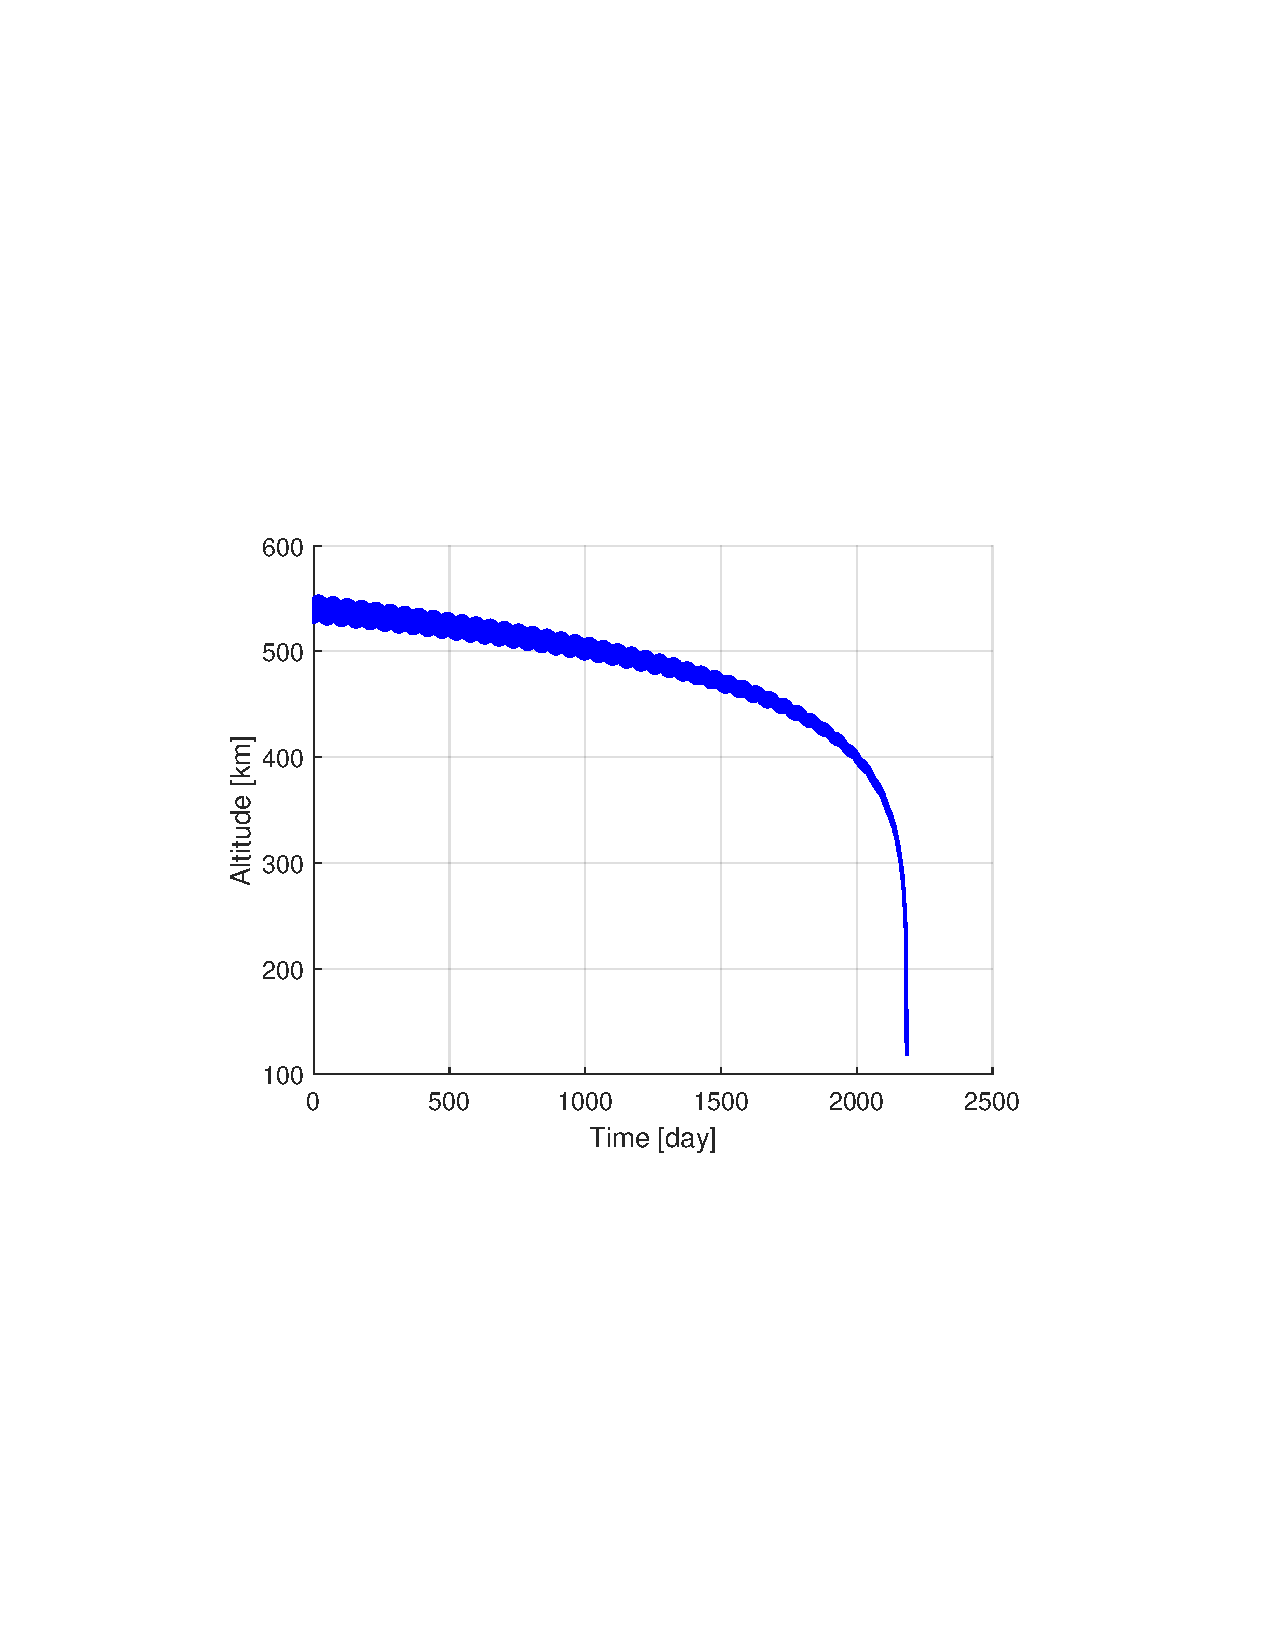
\includegraphics[trim=3.5cm 8cm 4.0cm 8cm,clip, width=0.8\textwidth]{curves/Altitude.pdf}
        \caption{Lifetime analysis.}
        \label{fig:lifetime-analysis}
    \end{center}
\end{figure}

\subsection{Ground Station Passes and Data Transfer Analysis}

Considering two ground stations, one at the SpaceLab installations in Florianópolis (27$^{\circ}$ 36' 00.9" S, 48$^{\circ}$ 31' 03.2" W) and other at the INPE/CRN installations in Natal (5$^{\circ}$ 50' 10.1" S, 35$^{\circ}$ 12' 27.5" W), both with a minimum elevation of 15$^{\circ}$, the results in \autoref{tab:grs-contacts-analysis}) were achieved. %during the simulations on GMAT .

\begin{table}[!h]
    \centering
    \begin{tabular}{lccc}
        \toprule[1.5pt]
        \textbf{Parameter} & \textbf{UFSC Station} & \textbf{INPE-RN Station} & \textbf{Unit} \\
        \midrule
        Minimum elevation to a valid contact    & 15    & 15    & $^{\circ}$ \\
        Number of contacts                      & 143   & 125   & - \\
        Minimum contract period                  & 24    & 34    & sec \\
        Maximum contact period                  & 395   & 394   & sec \\
        Average contact period                  & 303   & 298   & sec \\
        Total contact period                    & 43394 & 37205 & sec \\
        \bottomrule[1.5pt]
    \end{tabular}
    \caption{Ground station contacts analysis during the first 60 days of operation.}
    \label{tab:grs-contacts-analysis}
\end{table}

As seen from \autoref{tab:grs-contacts-analysis}, during the first 60 days of operation, considering the two main ground stations that will contact the satellite, the total contact period is 80599 seconds (43394 + 37205). With the data rate of the downlink/uplink as 4800 bps, this period will allow a data transfer of 48359400 bytes (or 46.12 M$_{i}$B) between GOLDS-UFSC and the Earth. Using the satellite's lifetime from the previous analysis (2000 days), and an average data transfer per day of 805990 bits, the total theoretical raw data transfer during the whole operation of the satellite will be approximately 1.5 G$_{i}$B.

These values can be even more significant if a smaller minimum elevation is considered, or with more ground stations in other locations.

\section{Mass Budget} \label{mass-budget}

The mass budget of the satellite can be seen in \autoref{tab:mass-budget}.

\begin{table}[!h]
    \centering
    \begin{tabular}{llc}
        \toprule[1.5pt]
        \textbf{Subsystem} & \textbf{Model} & \textbf{Mass [g]} \\
        \midrule
        OBDH                        & SpaceLab OBDH 2.0             & 53 \\
        TTC                         & SpaceLab TTC 2.0              & 52 \\
        EPS                         & SpaceLab EPS 2.0              & 80 \\
        Battery                     & SpaceLab Battery Module 4C    & 235 \\
        Antenna                     & ISISpace AntS                 & 89 \\
        ACS                         & SpaceLab Passive ACS 2U       & 100 (TBC) \\
        Payload                     & INPE-RN EDC                   & 75 ($\times$2) \\
        Radiation instrument            & SpaceLab Payload X            & 75 (TBC) \\
        Interface                   & SpaceLab Interface Boards     & 40 \\
        PC-104 Adapter              & SpaceLab PC-104 Adapter       & 50 (TBC) \\
        Solar Panel                 & Orbital Custom Solar Panel    & 266 \\
        Shields                     & 3 mm aluminum sheets          & 590 (TBC) \\
        Structure                   & Usiped Custom 2U Structure    & 206 \\
        Cables                      & -                             & 200 \\
        Others                      & -                             & 100 \\
        \midrule
        Total                       & -                             & \textbf{2211} \\
        Max. CubeSat 2U             & -                             & 2666 \\
        Margin                      & -                             & 455 \\
        \bottomrule[1.5pt]
    \end{tabular}
    \caption{Mass budget of the satellite.}
    \label{tab:mass-budget}
\end{table}

According to the CubeSat standard \cite{cds}, the maximum mass of each unit must be 1.33 kg. As the GOLDS-UFSC is a 2U CubeSat, the maximum allowed mass of the project is 2.66 kg. Considering the weight of each subsystem presented in \autoref{tab:mass-budget}, the current total mass of the object is below the maximum allowed, with a margin of 16 \%.

\section{Power Budget} \label{power-budget}

According to section 10.3 of \cite{larson2005}, the power budget of a satellite can be determined through three steps:

\begin{enumerate}
    \item Prepare operating power budget
    \item Size the battery
    \item Estimate power degradation over mission life
\end{enumerate}

\subsection{Input Power}

Simulations of the energy input to the solar panels along some orbits can be seen in the \autoref{fig:sp_sim_power} graph. Two extreme orbit scenarios, without and with maximum eclipse, were tested. The figures show the power generated on each side of the CubeSat, as well the total and average values.

\begin{figure}[!htb]
    \begin{center}
        \subfigure[Maximum eclipse.\label{fig:max_eclipse}]
        {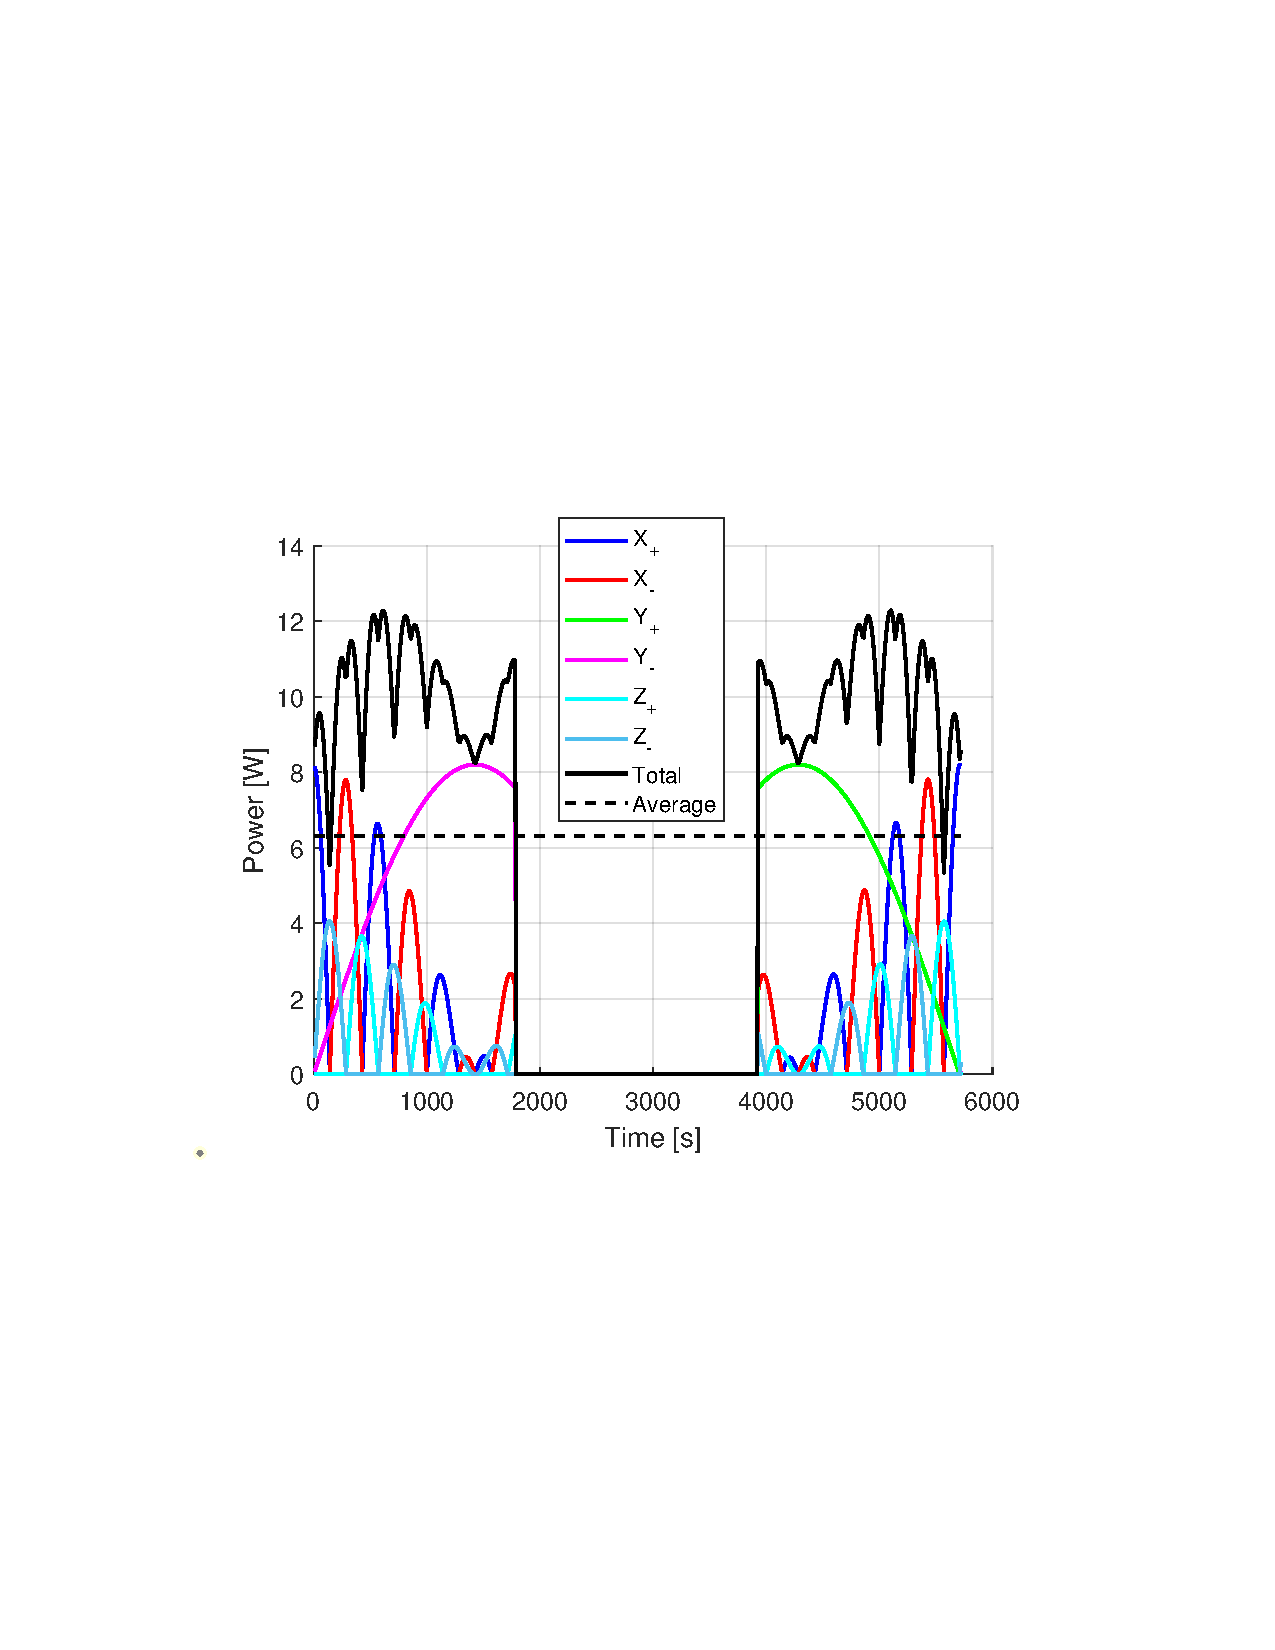
\includegraphics[trim=4cm 8.5cm 4cm 8.5cm, clip, width=0.45\textwidth]{curves/GOLDS_com_eclipse.pdf}}
        ~
        \subfigure[Without eclipse.\label{fig:without_eclipse}]
        {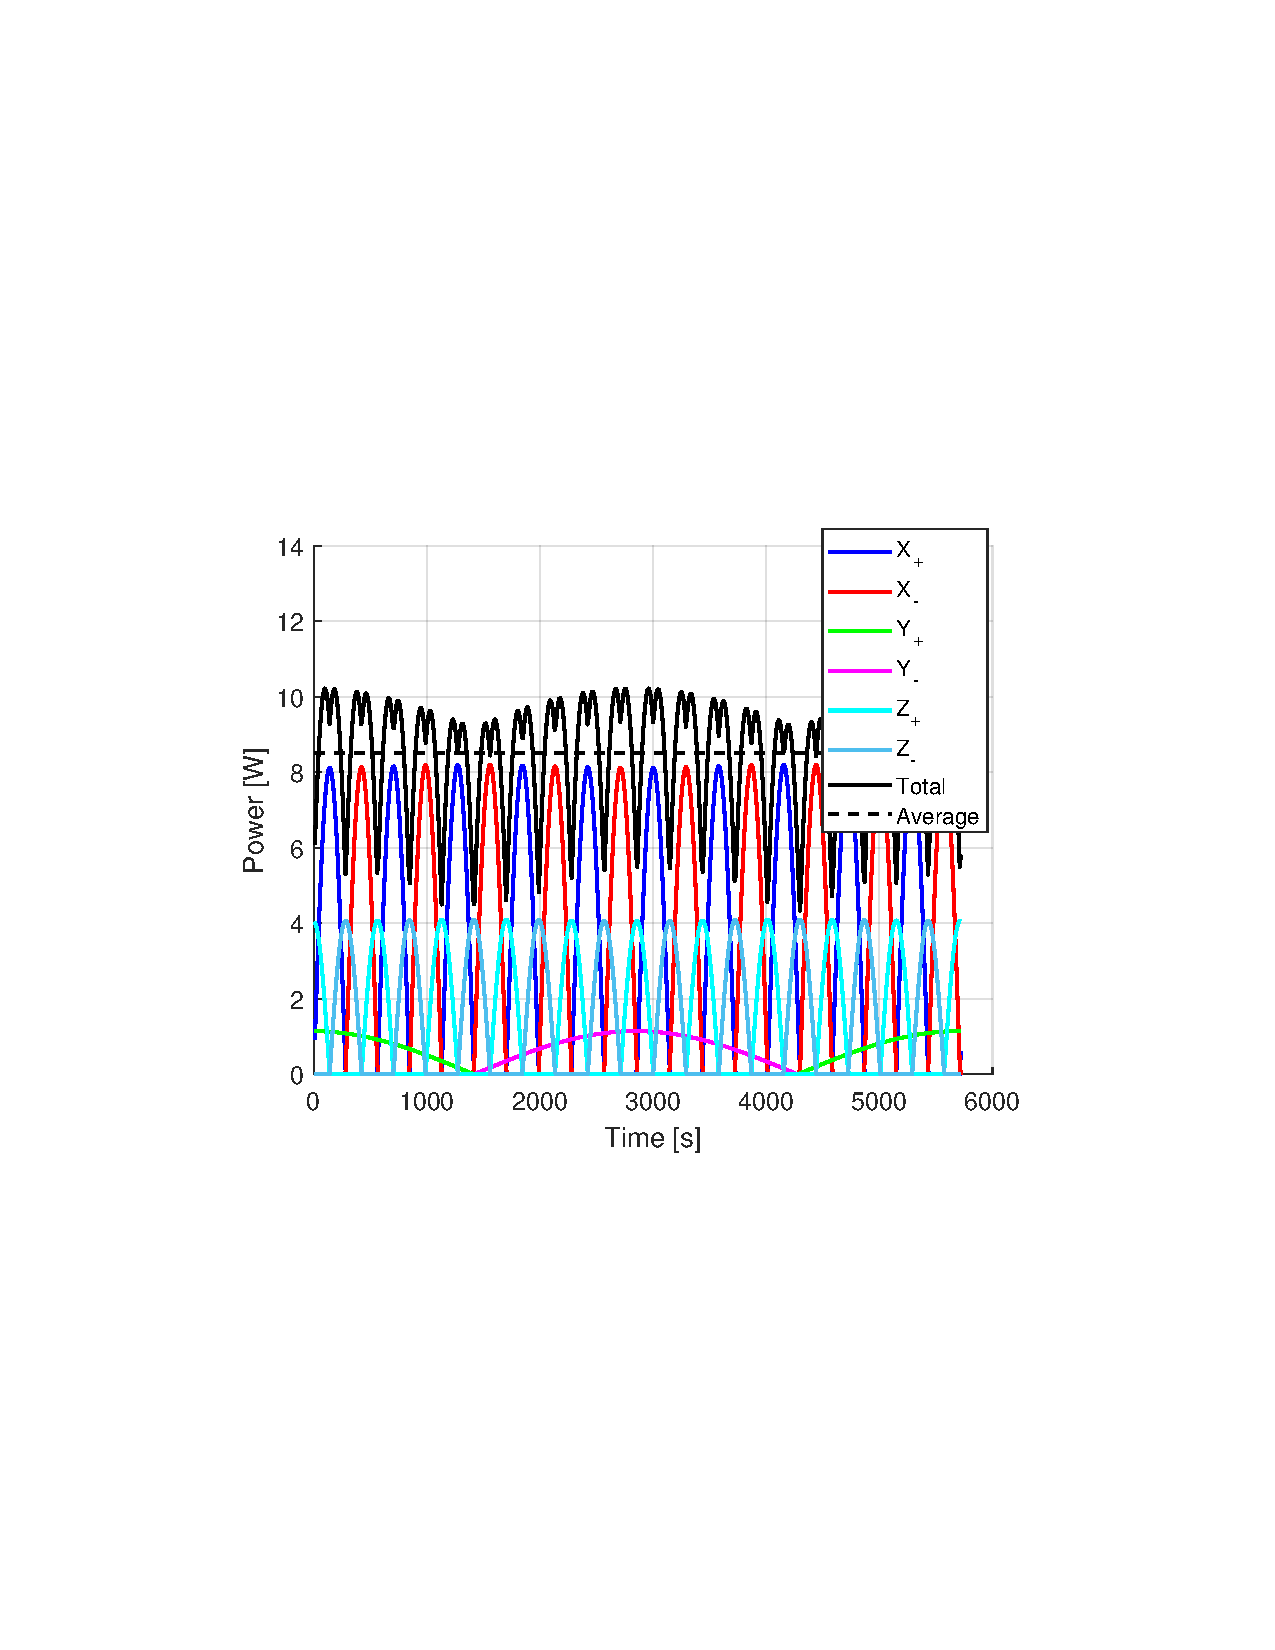
\includegraphics[trim=4cm 8.5cm 4cm 8.5cm, clip, width=0.45\textwidth]{curves/GOLDS_sem_eclipse.pdf}}
        \caption{Simulated input power of the solar panels.}
        \label{fig:sp_sim_power}
    \end{center}
\end{figure}

From these simulations, the results in \autoref{tab:power-simulations} were obtained:

\begin{table}[!htb]
    \centering
    \begin{tabular}{lcc}
        \toprule[1.5pt]
        \textbf{Parameter} & \textbf{Maximum eclipse} & \textbf{Without eclipse} \\    \midrule
        Peak power & 12282.7 mW & 10217.2 mW\\
        Average power (total orbit) & 6306.9 mW & 8519.6 mW \\
        Average (sunlight) & 10048.9 mW & 8519.6 mW\\
        Orbit period & 5720 s & 5720 s \\
        Sun light period &  3590 s & 5720 s\\
        Eclipse period & 2130 s & 0 s \\
        \bottomrule[1.5pt]
    \end{tabular}
    \caption{Results for the power input.}
    \label{tab:power-simulations}
\end{table}


\subsection{Operating Power Budget}

Typical operating voltages and current and power ranges consumed by each satellite subsystem are presented in \autoref{tab:power-requirements}.

\begin{table}[!h]
    \centering
    \begin{tabular}{lccccc}
        \toprule[1.5pt]
        \multirow{2}{*}{\textbf{Module}} & \multirow{2}{*}{\textbf{Voltage [V]}}    & \multicolumn{2}{c}{\textbf{Current [mA]}} & \multicolumn{2}{c}{\textbf{Power [mW]}} \\
                                         &                                          & \textbf{Min.} & \textbf{Max.}             & \textbf{Min.} & \textbf{Max.} \\
        \midrule
        OBDH                & 3.3   & 35    & 200   & 115   & 660 \\
        TTC ($\mu$C)        & 3.3   & 40    & 40    & 132   & 132 \\
        TTC (radio module)  & 5     & 10    & 650   & 33    & 3250 \\
        EPS (digital part)  & 7.4   & 50    & 260   & 165   & 858 \\
        EPS (heater)        & 7.4   & 675   & 675   & 5000  & 5000 \\
        Antenna module      & 3.3   & 60    & 550   & 200   & 1800 \\
        Payload EDC         & 5     & 250   & 250   & 1250  & 1250 \\
        Radiation instrument           & 5     & TBD   & TBD   & TBD   & TBD \\
        \bottomrule[1.5pt]
    \end{tabular}
    \caption{Power requirements of the subsystems and payloads of the satellite.}
    \label{tab:power-requirements}
\end{table}

Using the information presented in \autoref{tab:power-requirements}, and the activation periods defined for each module (the duty cycle), we arrive at the average satellite consumption present in \autoref{tab:power-consumption}.

\begin{table}[!h]
    \centering
    \begin{tabular}{lccccc}
        \toprule[1.5pt]
        \textbf{Module} & \textbf{Duty Cycle [\%]}    & \textbf{Power [mW]} \\
        \midrule
        OBDH                    & 100   & 115 \\
        TTC (radio 1 RX)        & 95    & 65 \\
        TTC (radio 1 TX)        & 5     & 3250 \\
        TTC (radio 2 RX)        & 95    & 65 \\
        TTC (radio 2 TX)        & 5     & 3250 \\
        EPS                     & 100   & 320 \\
        BAT (idle)              & 90    & 0 \\
        BAT (heater full)       & 10    & 5000 \\
        Antenna (deployment)    & 0     & 1800 \\
        Antenna (deployed)      & 100   & 35 \\
        Payload EDC             & 100   & 1250 \\
        Radiation instrument        & 0     & 1000 \\
        \cmidrule{2-3}
        Satellite               & \multicolumn{2}{c}{$\cong$ 2668} \\
        \bottomrule[1.5pt]
    \end{tabular}
    \caption{Power consumption of the subsystems and payloads of the satellite.}
    \label{tab:power-consumption}
\end{table}

The duty cycles of \autoref{tab:power-consumption} were defined according to the following assumptions:

\begin{itemize}
    \item One of the EDC payload is always off (cold redundancy).
    \item The Radiation instrument is turned on just during limited periods and only with telecommands.
\end{itemize}

As can be seen from \autoref{fig:sp_sim_power} and \autoref{tab:power-consumption}, there is a slight positive margin of \textbf{76.9 mW} in the power budget.

\subsection{Battery Sizing}

As described in \cite{larson2005}, the battery sizing of a satellite can be made by following the steps below:

\begin{enumerate}
    \item Estimate power level that the battery must supply
    \item Compute discharge cycle duration, charge cycle duration, and numbers of charge-discharge cycles
    \item Select depth of discharge
    \item Select charge rate
    \item Compute battery recharge power
\end{enumerate}

The power level that the battery must supply is the total power consumption of the satellite and is available in \autoref{tab:power-consumption}.

The discharge and charge cycle duration can be obtained from \autoref{fig:sp_sim_power}. The discharge duration is approximately 35.3 min (or 0.5889 h), and the charge cycle duration is 61.83 min (or 1.031 h). This is considering a single complete orbit.

The depth of discharge (DoD\nomenclature{\textbf{DoD}}{\textit{Depth of Discharge.}}) can be obtained using the \autoref{eq:dod-equation}.

\begin{equation} \label{eq:dod-equation}
    DoD = \frac{D_{i} \cdot D_{t}}{C} \cdot 100\ \%
\end{equation}

Where:

\begin{itemize}
    \item $D_{i}$: Discharge rate
    \item $D_{t}$: Discharge period
    \item $C$: Battery capacity
\end{itemize}

As the battery cells are already selected (5000 mAh in total, as described in \autoref{ssec:battery-module}), the current DoD is computed in \autoref{eq:dod-value}.

\begin{equation} \label{eq:dod-value}
    DoD = \frac{2668\ mW \cdot 0.5889\ h}{18500\ mWh} \cdot 100 \cong \mathbf{8.5\ \%}
\end{equation}

The charge rate can be estimated from the power input of the solar panels when the satellite is in sunlight. As presented before, the simulation results estimate the power input as 4315.6 mW. Considering the charge time as 61.83 min (or 1.031 h), the input energy is 4450 mWh. From \autoref{tab:power-consumption}, the power consumption of the satellite at sunlight is 2169 mW (or 2236 mWh considering the sunlight period). This way, energy input at sunlight is obtained in \autoref{eq:energy-input-sun-light}.

\begin{equation} \label{eq:energy-input-sun-light}
    4450 - 2236 = 2214\ mWh
\end{equation}

From the DoD calculation, the energy consumption during the eclipse is 1571 mWh. This way, the energy margin of the battery becomes positive ($2214 - 1571 = 643 mWh$), as expected from the power budget results.

All results from the battery sizing are available in \autoref{tab:battery-sizing-results}.

\begin{table}[!h]
    \centering
    \begin{tabular}{lcc}
        \toprule[1.5pt]
        \textbf{Parameter} & \textbf{Value}    & \textbf{Unit} \\
        \midrule
        Battery capacity                & 18500  & mWh \\
        Energy consumption on sunlight & 2169   & mWh \\
        Energy consumption on eclipse   & 1571   & mWh \\
        Sunlight duration              & 1.031  & h \\
        Eclipse duration                & 0.5889 & h \\
        Depth of Discharge (DoD)        & 8.5    & \% \\
        Total battery energy margin     & 643    & mWh \\
        \bottomrule[1.5pt]
    \end{tabular}
    \caption{Battery sizing results.}
    \label{tab:battery-sizing-results}
\end{table}

From the results, the battery sizing is well suited for the current satellite configuration and the planned behavior.

\subsection{Power Degradation Over Mission Life}

Two major events along the satellite operation should be considered in the power degradation analysis:

\begin{enumerate}
    \item Solar panels degradation
    \item Battery degradation
\end{enumerate}

From \cite{larson2005}, 5 \% per year is a usual number for the solar panels' degradation, in other words, the general efficiency of the solar panels decays at a rate of 5 \% per year of operation.% Also, \cite{larson2005} defines the battery degradation (or aging )as XX \% per year.

%A partial discharge reduces stress and prolongs battery life, so does a partial charge. Elevated temperature and high currents also affect cycle life

\section{Link Budget}

The link budget of all satellite radio links is available in \autoref{tab:link-budget-results}.

\begin{table}[!h]
    \centering
    \begin{tabular}{L{0.3\textwidth}ccccc}
        \toprule[1.5pt]
        \textbf{Variable} & \textbf{Beacon} & \textbf{Downlink} & \textbf{Uplink} & \textbf{Uplink (Payload)} & \textbf{Unit}\\
        \midrule
        Altitude                        & 550           & 550           & 550           & 550           & km \\
        Elevation                       & 0             & 0             & 0             & 0             & $^{\circ}$ \\
        Frequency                       & 146           & 450           & 450           & 401.635       & MHz \\
        Modulation                      & GMSK          & GMSK          & GMSK          & BPSK          & - \\
        Protocol                        & NGHam         & NGHam         & NGHam         & SBCD          & - \\
        Transmit power                  & 30            & 30            & 44            & 30            & dBm \\
        Transmitter antenna gain        & 0             & 0             & 12            & 3             & dBi \\
        Receiver antenna gain           & 12            & 12            & 0             & 0             & dBi \\
        FSPL                            & 144.4         & 154.2         & 154.2         & 153.2         & dB \\
        Power at receiver               & -107.4        & -117.2        & -103.16        & -125.2        & dBm \\
        Receiver sensibility            & -134          & -134          & -126          & -128          & dBm \\
        System losses                   & 5             & 5             & 5             & 5             & dB \\
        Receiver noise temp.            & 361.7         & 361.7         & 361.7         & 361.7         & K \\
        Antenna noise temp.             & 300           & 300           & 300           & 300           & K \\
        System noise temp.              & 661.7         & 661.7         & 661.7         & 661.7         & K \\
        Data rate                       & 1200          & 9600          & 9600          & 400           & bps \\
        Received SNR                    & 32.22         & 13.41         & 27.41         & 19.17         & dB \\
        SNR required for $10^{-5}$ BER\footnotemark & 9.6           & 9.6           & 9.6           & 9.6           & dB \\
        Link margin                     & $\geq$ 22.62  & $\geq$ 3.812  & $\geq$ 17.81  & $\geq$ 9.57   & dB \\
        \bottomrule[1.5pt]
    \end{tabular}
    \caption{Link budget results.}
    \label{tab:link-budget-results}
\end{table}

\footnotetext{Without FEC\nomenclature{\textbf{FEC}}{\textit{Forward Error Correction.}}.}

As can be seen, considering the worst case for the estimated orbit, that is, with the satellite on the horizon and with an elevation of zero degrees, the margin of all links is positive with a considerable balance.

All equations and steps used to obtain the results of \autoref{tab:link-budget-results} are available in \autoref{anx:link-budget}.
